\documentclass[10pt,twocolumn]{article}

%%% packages %%%
\usepackage{color}
\usepackage{graphicx}
\usepackage{listings}
\usepackage{float}
\usepackage{url}
\usepackage{times}
\usepackage{xspace}
\usepackage{microtype}
\begin{document}

\title{Profile-guided Optimization\ \\
  \small CSE 501 Spring 2013 Compilers Assignment 3}
\author{Andre Baixo, Jacob Nelson}
\maketitle

In this assignment, we implemented profile-guided function inlining.

Our static optimizations, implemented in the previous homework, did not
produce the correct result for some of the benchmarks. We started this
work by fixing \emph{all} the static optimizations, which now produce
the correct output for all the benchmarks used, including richards.

On top of this, we instrumented function calls, basic blocks and
dynamic load and store instructions, which are the most expensive
operations. The goal was to implement profile-guided function inlining and type speculation.

The results show that profile-guided optimizations can considerably improve performance
after static optimizations are applied.

\paragraph{Function inlining}
By counting the number of times that each call instruction is executed, it is possible to inline any call that is executed more times than a determined threshold. According to our experiments, a threshold of 6 calls yields the best speedup for /texttt{richards} benchmark, which is the application that benefits the most from inlining. Other benchmarks face negligible speedups or slowdowns, while \texttt{richards} have a 13\% speedup due to function inlining.

Function inlining is implemented as follows. First we detect the calls that were executed a number of times above the threshold. For each of these calls, if the called function is not the same that is calling (i.e. if caller and callee are not the same), the callee is inlined. If the inlined function itself has calls that were executed above the threshold, these are also inlined, as long as they do not introduce a call cycle.

For inlining the function we first create a number of local variables in the caller equal to the number of local variables in the callee plus the number of parameters necessary for calling it. For this, we simply update the header of the caller function (we copy the types from the header of the called function), and then we update the \emph{enter} instruction of the caller to allocate space for the additional local variables.

After this, we replace the \emph{param} instructions that preceed the call that will be inlined by \emph{move}s to the newly created local variables. The callee function is then
inlined, removing its last \emph{ret} instructions and replacing each of the other \emph{ret}s that might be present in the callee by a branch to the intruction that comes after
the call that is being replaced in the caller (this instruction is also the new target of any callee instruction that jump to the callee's final \emph{ret}.) Finally, every reference to a register, variable, parameter or target is updated to reflect the new position of the code.

\paragraph{Type speculation}

Load and store dynamic are by far the most expensive instructions in
the interpreter. For this reason, we attempted an implementation of
type speculation for load and store dynamic
instructions. Unfortunately, we were not able to debug this
optimization in time.

To apply this optimization, we collected type occurence data for each
load or store dynamic instruction as discussed in the assignment, and
then used this data to add a special case for the most common type
used in each instruction instance. This special case would assume the
type was the expected one, and would speculatively compute the field
offset and load the filed data before testing the type and branching
to a recovery path that applied the dynamic instruction. 

One complexity in making this work is that the load dynamic
instruction automatically boxes integer fields; even when the field is
a raw integer, the instruction returns a pointer to a boxed
integer. This required us to add a special case to the optimization to
create a new boxed integer and fill in the value with the one we
loaded.

Figure~\ref{fig:hammock} shows an example from \texttt{class.dart}. In this
case we are loading a native integer field y from an object b of type
B. Instructions 37--39 are the same in the optimized and unoptimized
cases: they compute a pointer to b, load it and check that the result
is not null. Instruction 40 starts the optimization---we test whether
the loaded object is of type B. Then in instructions 41 and 42, we
speculatively compute the y field offset and load the data. Since this
is a raw integer, we must box it, so instructions 43--45 creates a new
boxed integer and store the loaded data into i. Finally in instruction
46, we store the pointer to the boxed integer into a temporary variable. 

Instruction 47 uses the result of the type check to branch to the
dynamic fallback case in BB 91. When the type doesn't match our
speculation, we run the standard dynamic instruction and store the
result into our temporary variable. 

Finally, the result of the optimization is used in instruction 48.

\begin{figure}
\begin{center}
  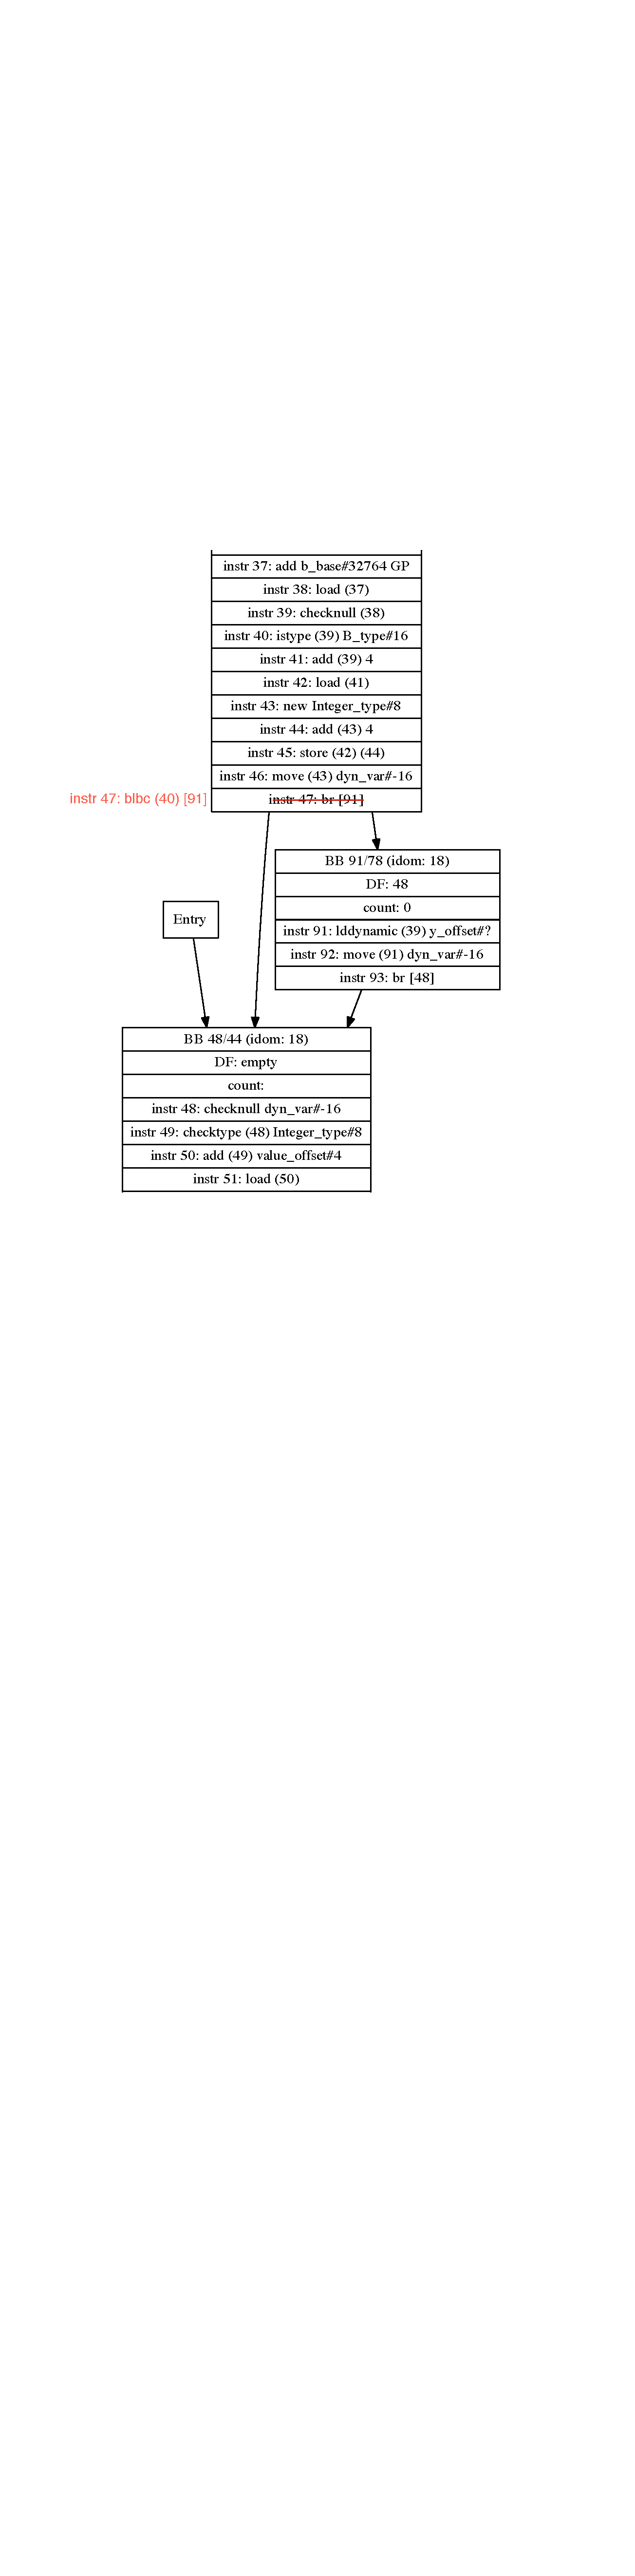
\includegraphics[width=0.95\columnwidth]{figs/class-example.pdf}
\begin{minipage}{0.95\columnwidth}
  \caption{\label{fig:hammock} Type speculation example.}
\end{minipage}
\end{center}
\end{figure}

Unfortunately there are still bugs in this implementation: when we run
it on \texttt{class.dart}, we see a 20 percent speedup, but we also get the
wrong answer.

\section{Performance}

Table~\ref{results} shows the number of cycles needed to execute the five
most interesting benchmarks. Notice that, except for \texttt{mmm}, the benchmarks listed exhibit a slowdown
after performing simple constant propagation and global common subexpression elimination.
The reason is probably that dead code elimination is not performed in order
to get rid of unecessary copies introduced by both the static optimizations and the translation
back from the SSA form. For \texttt{mmm} though, function inlining introduced some slowdown.
Other benchmarks not listed experienced some speedup from static optimizations without any
slowdown from inlining, as no call was inlined.

On the other hand, profile-guided function inlining improves performance for all the benchmarks, except for \texttt{mmm}.
In fact, except for the \texttt{hanoifibfac} benchmark, function inlining overcomes the slowdown
introduced by the static optimizations and surpass the unoptimized code. For \texttt{hanoifibfac}, inlining does improve
performance, but it's not enough to overcome the slowdown introduced by the static optimizations.

\begin{table}
\begin{tabular}{|l|l|l|l|} \hline
~           & \textbf{Unoptmized} & \textbf{scp + cse}  & \textbf{scp + cse + inlining} \\ \hline
cproptest   & 227        & 230        & 221                  \\ \hline
hanoifibfac & 4548       & 5750       & 5416                 \\ \hline
mmm         & 7371       & 7229       & 7777                 \\ \hline
richards    & 26,933,770 & 29,493,534 & 25,840,024           \\ \hline
vnumtest    & 537        & 541        & 466                  \\ \hline
\end{tabular}
\caption{Performance results in number of cycles.}
\label{results}
\end{table}


\section{Running}

The optimizer may be run by executing the \texttt{assignment2/run.sh}
script while inside the \texttt{assignment2} directory. We have
included precompiled intermediate languages files for all examples in
the distribution. Running the script will create separate output files
in the \texttt{examples} directory for each method of each example;
optimized intermediate language output has the extension
\texttt{.ilo}, dump information has the extension \texttt{.txt}, and
CFG output has the extension \texttt{.dot}. For example, the optimized
IL for \texttt{gdc.dart} can be found in
\texttt{examples/gcd.dart.ilo}. The GraphViz files can be turned into
PDF with a command like \texttt{dot -Tpdf file.dot > file.pdf}.

The script mostly follows the interface described in the assignment;
optimizations are selected by specifying a comma-separated list to the
\texttt{-opt=} flag, and similarily backends with the
\texttt{-backend=} flag. We write output to files as specified above
instead of stdout, since there is often a lot of output. There is a
new \texttt{-profile=} flag to specify counter output from the
interpreter for applying profile-guided optimizations.

Choices for optimization include \texttt{ssa}, \texttt{scp},
\texttt{cse}, and \texttt{profile}. Using the \texttt{profile} option
will add profiling instrumentation to the generated code.

Choices for backend include SSA deconversion, \texttt{ssa}; IL output,
\texttt{ir}; CFG output, \texttt{cfg}. Reports are disabled in this
version.

To apply profile-guided optimizations, first run with
-opt=ssa,cse,scp,profile. When you run the program under start with
stats enabled, you will get counter output. Copy just the counters
into a .prof file (a few are included in the assignment2 directory),
and rerun the compiler with -opt=ssa,cse,scp and
-profile=[filenamee]. This will generate a new .ilo file with the
profile-guided optimizations applied.

Our optimizer is implemented in Ruby, so no separate build step is
required. Ruby version 1.9 is required. 




\bibliographystyle{abbrv}
\bibliography{writeup}

\end{document}

